\documentclass[12pt]{report}
%====================== PACKAGES ======================
\usepackage[french]{babel}
\usepackage[utf8x]{inputenc}
%pour gérer les positionnement d'images
\usepackage{float}
\usepackage{amsmath}
\usepackage{graphicx}
\usepackage[colorinlistoftodos]{todonotes}
\usepackage{url}
%pour les informations sur un document compilé en PDF et les liens externes / internes
\usepackage{hyperref}
%pour la mise en page des tableaux
\usepackage{array}
\usepackage{tabularx}
%pour utiliser \floatbarrier
%\usepackage{placeins}
%\usepackage{floatrow}
%espacement entre les lignes
\usepackage{setspace}
%modifier la mise en page de l'abstract
\usepackage{abstract}
%police et mise en page (marges) du document
\usepackage[T1]{fontenc}
\usepackage[top=2cm, bottom=2cm, left=2cm, right=2cm]{geometry}
%Pour les galerie d'images
\usepackage{subfig}
\usepackage[utf8]{inputenc}
\usepackage{fancyhdr}
\usepackage[acronym]{glossaries} 
\pagestyle{fancy}
\fancyhf{}
\fancyhead[LE,RO]{2021}
\fancyhead[RE,LO]{Projet de JAVA EE}
\fancyfoot[CE,CO]{\leftmark}
\fancyfoot[LE,RO]{\thepage}
\pagenumbering{arabic}

\renewcommand{\headrulewidth}{2pt}
\renewcommand{\footrulewidth}{1pt}
%====================== INFORMATION ET REGLES ======================

%rajouter les numérotation pour les \paragraphe et \subparagraphe
\setcounter{secnumdepth}{4}
\setcounter{tocdepth}{4}

\hypersetup{							% Information sur le document
pdfauthor = {Premier Auteur,
			Deuxième Auteur,
			Troisième Auteur,
    		Quatrième Auteur},			% Auteurs
pdftitle = {Nom du Projet -
			Sujet du Projet},			% Titre du document
pdfsubject = {Mémoire de Projet},		% Sujet
pdfkeywords = {Tag1, Tag2, Tag3, ...},	% Mots-clefs
pdfstartview={FitH}}					% ajuste la page à la largueur de l'écran
%pdfcreator = {MikTeX},% Logiciel qui a crée le document
%pdfproducer = {}} % Société avec produit le logiciel

%======================== DEBUT DU DOCUMENT ========================
\makeglossaries
\begin{document}

%régler l'espacement entre les lignes
\newcommand{\HRule}{\rule{\linewidth}{0.5mm}}
\setcounter{page}{4}

%page de garde
\begin{titlepage}
	\vspace{0.8cm}
	\includegraphics[width=0.205\textwidth,left=5cm]{ensias.png}
	\hspace{8cm}
	\includegraphics[width=0.3\textwidth, right=25cm]{um5.png}
\begin{center}

% Upper part of the page. The '~' is needed because only works if a paragraph has started.


\textsc{\Large }\\[0.5cm]

% Title
	\vspace{2cm}	


	\LARGE
		\HRule\\[0.4cm]

	Rapport de Projet de JAVA EE:\\
	\vspace{1cm}
	\LARGE
		\includegraphics[width=0.5\textwidth, right=20cm]{logo.png}\\
    \vspace{1cm}
    \textbf{Application web de gestion de location de voiture}	\\
		
	\HRule\\[3cm]




% Author and supervisor
\begin{minipage}{0.4\textwidth}
\begin{flushleft} \large
\textbf{Réalisé par:}\\
\vspace{0.8cm}
TALHAOUI \textsc{Mouad}\\
RAMI \textsc{Anass}\\
TNIFASS \textsc{Mehdi}\\
MAADANI \textsc{khalil}\\

\end{flushleft}
\end{minipage}
\begin{minipage}{0.4\textwidth}
\begin{flushright} \large
\textbf{Encadré par:} \\
\vspace{0.8cm}
MAHMOUD \textsc{EL HAMLAOUI }\\

\end{flushright}
\end{minipage}
%\begin{minipage}{0.4\textwidth}
%\begin{center} \large
%\textbf{Jury:} \\
%\vspace{0.5cm}
%Bouchra \textsc{EL ASRI }\\
%Hatim  \textsc{Guermah}\\

%\end{center}
%\end{minipage}
\vspace{1cm}
\vfill

% Bottom of the page
2020/2021


\end{center}
\end{titlepage}

\newpage
~
\listoffigures

\listoftables


\thispagestyle{empty}
\newpage

\tableofcontents
\thispagestyle{empty}
\newpage
\chapter*{Remerciement}
\addcontentsline{toc}{chapter}{Remerciement}
\large
\begin{onehalfspace}
\large{	 Nous tenons, avant tout, à adresser nos plus vifs remerciements à Monsieur Mahmoud EL HAMLAOUI, notre cher encadrant de ce projet, qui nous a aidés à escamoter beaucoup de problèmes.
	 
	 Enfin, nos remerciements vont à tous les enseignants de l’École nationale supérieure d'informatique et d'analyse des systèmes, pour leurs aides et leur professionnalisme.}
\end{onehalfspace}
\chapter*{Introduction générale}
\addcontentsline{toc}{chapter}{Introduction}




\begin{onehalfspace}
\large{	 De nos jours, l’optimisation du temps et la bonne gestion de nos problèmes joue un rôle très important dans notre vie quotidienne afin d’escamoter beaucoup de problèmes.\\
	 
	 Dans ce contexte, nous proposons de présenter une application web nommée « Louezz » qui aide les différentes agences de location d’une part à trouver des clients, et les locateurs de voiture à chercher et trouver une voiture dans les plus brefs délais et le bon état possible.\\
	 
	 Le plan de ce rapport est composé de cinq chapitres :\\
	 
	 Le premier chapitre va présenter le projet de manière générale, la problématique et la solution proposée. Le deuxième chapitre est consacré à la présentation de l'analyse et la conception. Le troisième chapitre est réservé à la création de la base de données. Le quatrième chapitre est réservé à présentation des maquettes de projets. Le dernier chapitre présente les spécifications des environnements matériels et logiciels utilisées au cours du développement et aussi présente les différentes interfaces ainsi que les problèmes de programmation rencontrés.}
\end{onehalfspace}





\chapter{Présentation du projet}
\vspace{5cm}
\large{Ce premier chapitre présente tout d’abord d’une manière générale le projet et problématique liée à la résolution des problèmes et les déférentes raisons du choix de ce sujet de projet.\\}


\newpage
\section{Amenant}
\large{Au cours de notre formation en tant qu'Elève Ingénieur de l'ENSIAS en 2ème année, nous sommes appelés à travailler sur un projet Java EE à travers lequel nous exploitons nos connaisances et compétences acquis durant notre formation Développement et Ingéniere Web afin d'aboutir à une application Web basé complètement sur Java EE bien construite.\\
Avec l'accord de notre cher encadrant, nous avons choisi La Location de voiture comme sujet du projet.\\}
\section{Analyse de l'existant}
\large{De nos jours, l’optimisation du temps et la bonne gestion de nos problèmes joue un rôle très important dans notre vie quotidienne afin d’escamoter beaucoup de problèmes et face à la défaillance du système de transport ,le parc automobile marocain croît tous les ans avec son lot de désagréments : embouteillages, pollution, accident de la route. La location de voiture pourrait être la solution à tous ces soucis en réduisant le trafic, et en diminuant la pollution ainsi que la consommation d'énergie et la contribution des délais.\\

Ainsi au Maroc, les gens aujourd'hui optent pour cette alternative. Pour pallier aux problèmes liés à l'insuffisance de l'offre en matière du transport, à l'intérieur ou l'extérieur des villes, les Marocains prennent leurs maux en patience et innovent. Au sein des villes marocaines, face à l'anarchie régnante au sein du secteur du transport.\\

Au Maroc, avec l'émergence des technoligies ,les platformes  destinés à ce nouveau mode de transport sont très peu. Des centaines d'offres et de demandes sont publiées quotidiennement par les internautes, démontrant ainsi un réel engouement envers ce mode de transport destiné à pallier aux retards des trains, manque des moyens pour se procurer une voiture ou encore l'absence de confort de certains autocars.\\}
\section{Problématique soulevée}
La location de voiture n'est pas sans mésaventure. La location de voiture au Maroc échappe à toute surveillance. 
Par conséquent, deux problèmes majeurs trouvent chemin concernant la location du voiture au Maroc :\\

• \textbf{Relation entre agences et locateurs :}\\

Mettre en relation les agences de location et les locateurs et donner beaucoup d'information sur la voiture et l'agences.\\

• \textbf{L'organisation :}\\

Toute personne souhaitant reserver une voiture doit pouvoir trouver facilement grace a quelques cliques son but sans avoir à parcourir plusieurs pages.\\

\section{Solution proposée}
De ce qui précède, nous nous sommes aperçus que le besoin du palatforme de gestion de location de voiture au Maroc, étant un besoin nécessaire et important, est à saisir et mérite une profonde réfexion aux problèmes cités avant. Ainsi, nous l'avons associé à notre projet JEE pour aboutir une application Web dont les objectifs sont :\\

• \textbf{Assurer la location de voiture :}\\

mettre en relation les agences de location et les locateurs.\\


• \textbf{Assurer l'organisation :}\\

établir une app Web intuitive qui va interagir avec le visiteur en toute simplicité sans avoir à parcourir plusieurs pages, seulement avec quelques cliques .\\

\chapter{Analyse et Conception}
\vspace{5cm}
\large{Ce deuxième chapitre présente tout d’abord d’une manière générale La méthode que nous avons adopté pour réaliser l'analyse et la conception de notre système d'information.\\}


\newpage
\section{Méthode adoptée}
\large{La méthode que nous avons adopté pour réaliser l'analyse et la conception de notre système d'information est la méthode UML : Elle permet la séparation entre les données et les traitements effectués en plusieurs modèles conceptuels qui sont répartis sur 3 diagrammes : Le diagramme de cas d'utilisation, le diagramme de classe,diagramme de séquence. Dans cette partie, nous allons présenter quelques-unes de ces méthodes, et en denissant par les maquettes. Cette phase a pour objectif de déduire la spécication de l'architecture du système.\\}
\section{Diagramme de cas d'utilisations}
\large{les diagrammes de cas d'utilisation modélisent le comportement d'un système et permettent de capturer les exigences du système. Les diagrammes de cas d'utilisation décrivent les fonctions générales et la portée d'un système. Ces diagrammes identident également les interactions entre le système et ses acteurs. Les cas d'utilisation et les acteurs dans les diagrammes de cas d'utilisation décrivent ce que le système fait et comment les acteurs l'utilisent, mais ne montrent pas comment le système fonctionne en interne.}

%\subsection{Admin}
%\begin{page}{\textwidth}
%	\begin{page}{\linewidth}
%	\makebox[\linewidth]{
%		\includegraphics[keepaspectratio=true,scale=0.38]{uc1.jpeg}} 
%		\captionof{figure}{Diagramme de cas d'utilisation admin}\label{f3}%
%\end{page}
%\end{page}

\subsection{Utilisateur/visiteur}

\begin{page}{\textwidth}
	\begin{page}{\linewidth}
	\makebox[\linewidth]{
		\includegraphics[keepaspectratio=true,scale=0.38]{uc2.jpeg}} 
		\captionof{figure}{Diagramme de cas d'utilisation utilisateur/visiteur}\label{f3}%
\end{page}
\end{page}
\newpage
\section{Diagramme de classe}
\begin{page}{\textwidth}
	\begin{page}{\linewidth}
	\makebox[\linewidth]{
		\includegraphics[keepaspectratio=true,scale=0.9]{diagramme_de_classe.png}} 
		\captionof{figure}{Diagramme de classe}\label{f3}%
\end{page}
\end{page}
\newpage

\section{Diagramme de séquences}
\large{Pour schématiser la vue comportementale de notre système informatique, nous faisons recours au diagramme
de séquence d'UML. Ce diagramme permet de présenter les interactions entre l'acteur et le système avec des
messages présentés dans un ordre chronologique. Le diagramme de séquences traite le système informatique
comme étant une boite noire. Le comportement du système est décrit de l'extérieur sans avoir d'idée sur la
réalisation. Nous pouvons, alors, constater que certains cas d'utilisation sont similaires, c'est pourquoi nous
avons choisi de traiter quelques exemples.\\}

\newpage
\begin{figure}[p]

\centering
\includegraphics[width=1.3\textwidth, angle =90 ]{55.PNG}
\caption{Diagramme de séquence proposer une offre}
\label{fig:awesome_image}

\end{figure}
\newpage
\begin{figure}[p]

\centering
\includegraphics[width=1.3\textwidth, angle =90 ]{44.PNG}
\caption{Diagramme de séquence céer compte}
\label{fig:awesome_image}

\end{figure}
\newpage
\begin{figure}[p]

\centering
\includegraphics[width=1.3\textwidth, angle =90 ]{33.PNG}
\caption{Diagramme de séquence consulter les offres}
\label{fig:awesome_image}

\end{figure}
\newpage
\begin{figure}[p]

\centering
\includegraphics[width=1.3\textwidth, angle =90 ]{111.png}
\caption{Diagramme de séquence Choisir offre}
\label{fig:awesome_image}

\end{figure}
\newpage






\chapter{ Création de la base de données}
\vspace{5cm}
\large{Ce troisième chapitre st réservé à la création de la base de données.\\}


\newpage
\section{Shema de base de donnees}

\begin{minipage}{\linewidth}
	\makebox[\linewidth]{
		\includegraphics[keepaspectratio=true,scale=1.2]{data.PNG}}
	\captionof{figure}{shema de base de donnees}\label{f3}%    
\end{minipage}\\

\section{Signification de champs}
\begin{center}
\begin{table}[htp]

 \begin{tabular}{||c||  c||  c||  c||} 
 \hline
 Nom & ID & Type & Entite \\ [0.5ex] 
 \hline\hline
 identificateur de vehicule &  id\_vehicule & int & vehicule \\ 
 \hline
 Marque de vehicule & marque & varchar & vehicule \\
 \hline
 Modele de vehicule& modele & varchar & vehicule \\
 \hline
 
Type de carburant de vehicule& carburant & varchar & vehicule \\
 \hline
 
 kilometrage fait par le vehicule& kilometrage & int & vehicule \\
 \hline
  Type de vehicule& type\_vehicule & varchar & vehicule \\ 
 \hline
 photo1 de la vehicule& photo1 & varchar & vehicule \\
 \hline
 photo2 de la vehicule& photo2 & varchar & vehicule \\
 \hline
 Type de boite de vitesse& boite\_vitesse & varchar & vehicule \\
 \hline
 Nombre de places& nbr\_places & int & vehicule \\
 \hline
 Nombre de portes& nbr\_portes & int & vehicule \\
 \hline 
 ville & ville & varchar & vehicule \\
 \hline
 lieu de rencontre & lieu\_rencontre & varchar & vehicule \\
 \hline 
 Prix de l'offre& prix & int & vehicule \\
 \hline 
 Description de la vehicule& Descr & varchar & vehicule \\
 \hline 
 Date debut de disponibilite de vehicule& debut & date & vehicule \\
 \hline
 Date fin de disponibilite de vehicule&  fin & date & vehicule \\
 \hline 
 Etat de disponibilite de vehicule& etat & varchar & vehicule \\
 \hline
 Identificateur  de l'utilisater& id\_user & int & utilisateur \\
 \hline
 Nom  de l'utilisater& nom & varchar & utilisateur \\
 \hline
  Prénom  de l'utilisater& prenom & varchar & utilisateur \\
 \hline
 Date naissance  de l'utilisater & date\_naissance & date & utilisateur \\
 \hline
  Telephone  de l'utilisater& telephone & int & utilisateur \\
 \hline
 Adresse de l'utilisater & adresse\_utilisateur & varchar & utilisateur \\
 \hline 
 Login& login & varchar & utilisateur \\
 \hline 
 Email& email & varchar & utilisateur \\
 \hline 
 Mot de passe & password & varchar & utilisateur \\
 \hline 
 CIN & cin & varchar & utilisateur \\
 \hline 
  Numero de permis & num\_permis & varchar & utilisateur \\
 \hline 
  Photo de la vehicule& photo & varchar & utilisateur \\
 \hline 
  Identificateur de demande& id\_demande & int & demande \\
 \hline 
 Identificateur de utilisateur& id\_user & int & demande \\
 \hline 
  Identificateur de vehicule& id\_vehicule & int & demande \\
 \hline 
  Etat de traitement de demande & etat\_demande & varchar & demande \\
 \hline 


\end{tabular}
\caption{Signification de champs}
\end{table}
\end{center}

\chapter{Maquettes de projets}
\vspace{5cm}
\large{Ce quatrième chapitre est réservé à présentation des maquettes de projets.\\}


\newpage
\section{Maquette}
Une maquette est une représentation partielle ou complète d'un Système ou d'un objet (existant ou en projet) afin d'en tester et valider certains aspects et/ou le comportement (maquette fonctionnelle), ou simplement à des fins ludiques (maquette de jeu) ou informatives (présentation pédagogique ou commerciale d'une réalisation
ou d'un projet). Dans ce qui suit nous allons présenter les maquettes principales de notre site web .

\subsection{Maquette 1}
\begin{page}{\textwidth}
	\begin{page}{\linewidth}
	\makebox[\linewidth]{
		\includegraphics[keepaspectratio=true,scale=0.42]{Page_1.png}} 
		\captionof{figure}{Page d'acceuil}\label{f3}%
\end{page}
\end{page}

\subsection{Maquette 2}
\begin{page}{\textwidth}
	\begin{page}{\linewidth}
	\makebox[\linewidth]{
		\includegraphics[keepaspectratio=true,scale=0.42]{Page_3.png}} 
		\captionof{figure}{Créer un compte}\label{f3}%
\end{page}
\end{page}

\subsection{Maquette 3}
\begin{page}{\textwidth}
	\begin{page}{\linewidth}
	\makebox[\linewidth]{
		\includegraphics[keepaspectratio=true,scale=0.57]{Page_2.png}} 
		\captionof{figure}{Se connecter}\label{f3}%
\end{page}
\end{page}
\subsection{Maquette 4}
\begin{page}{\textwidth}
	\begin{page}{\linewidth}
	\makebox[\linewidth]{
		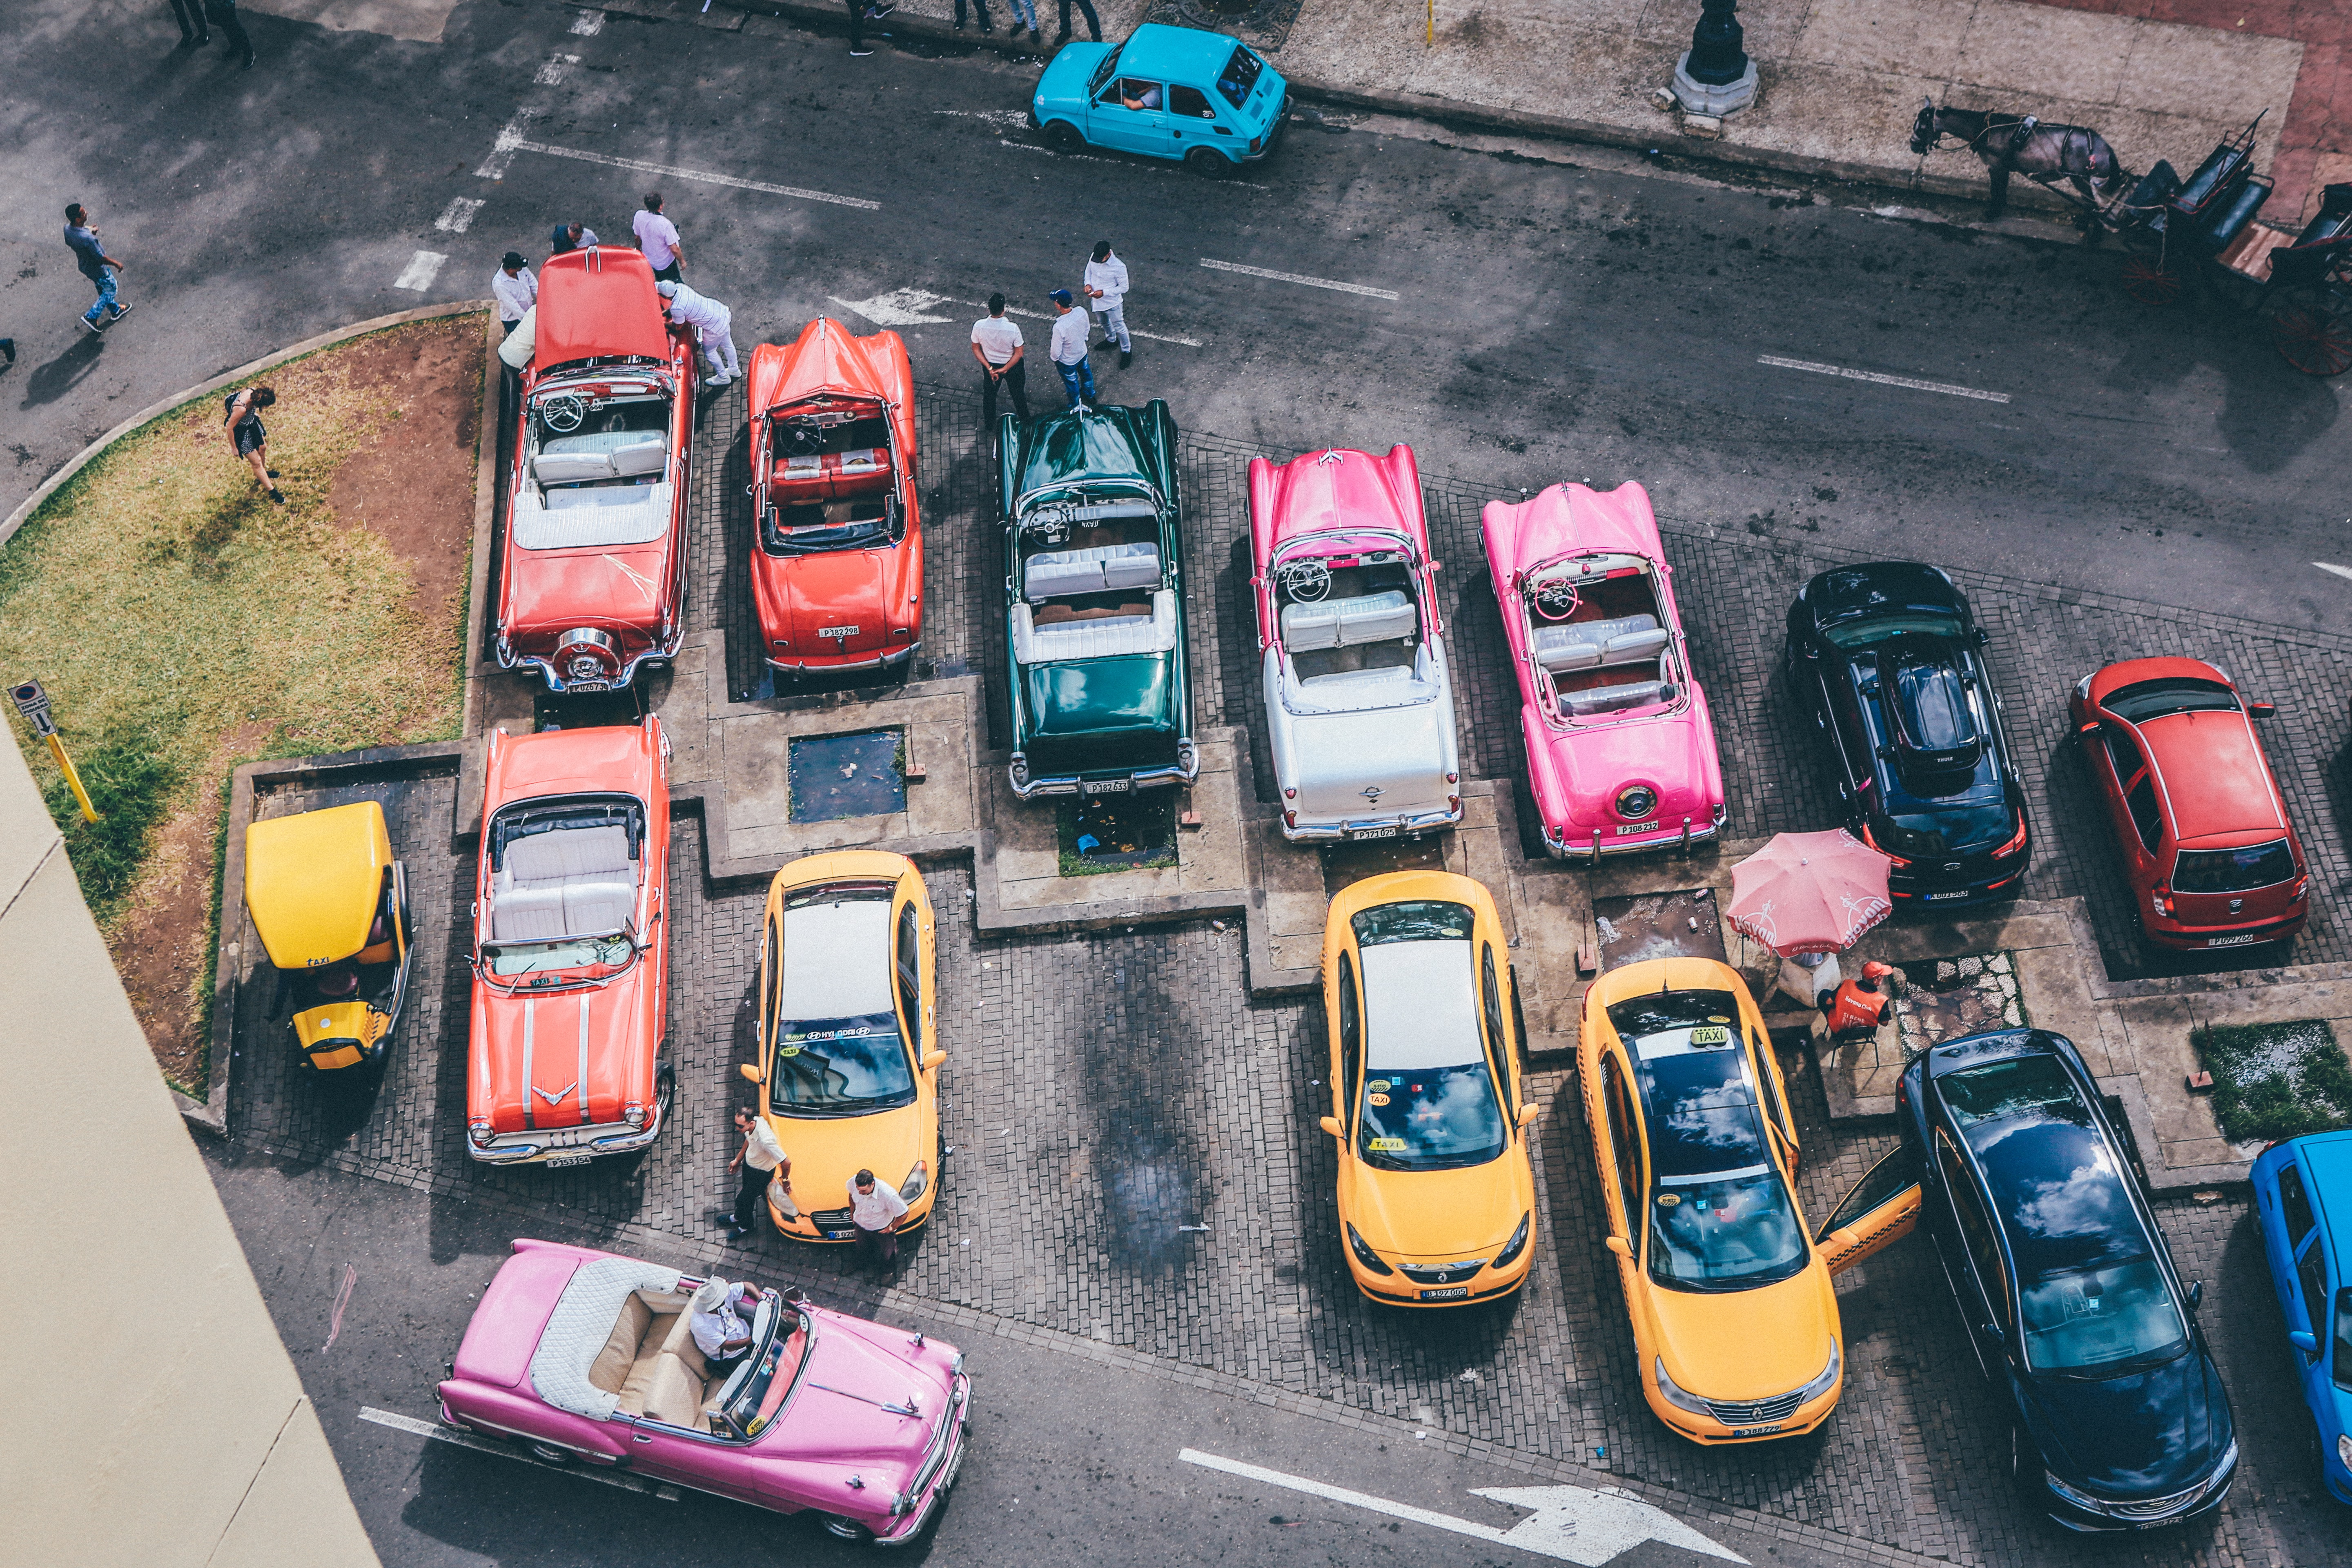
\includegraphics[keepaspectratio=true,scale=0.38]{1.png}} 
		\captionof{figure}{Page des offres}\label{f3}%
\end{page}
\end{page}
\subsection{Maquette 5}
\begin{page}{\textwidth}
	\begin{page}{\linewidth}
	\makebox[\linewidth]{
		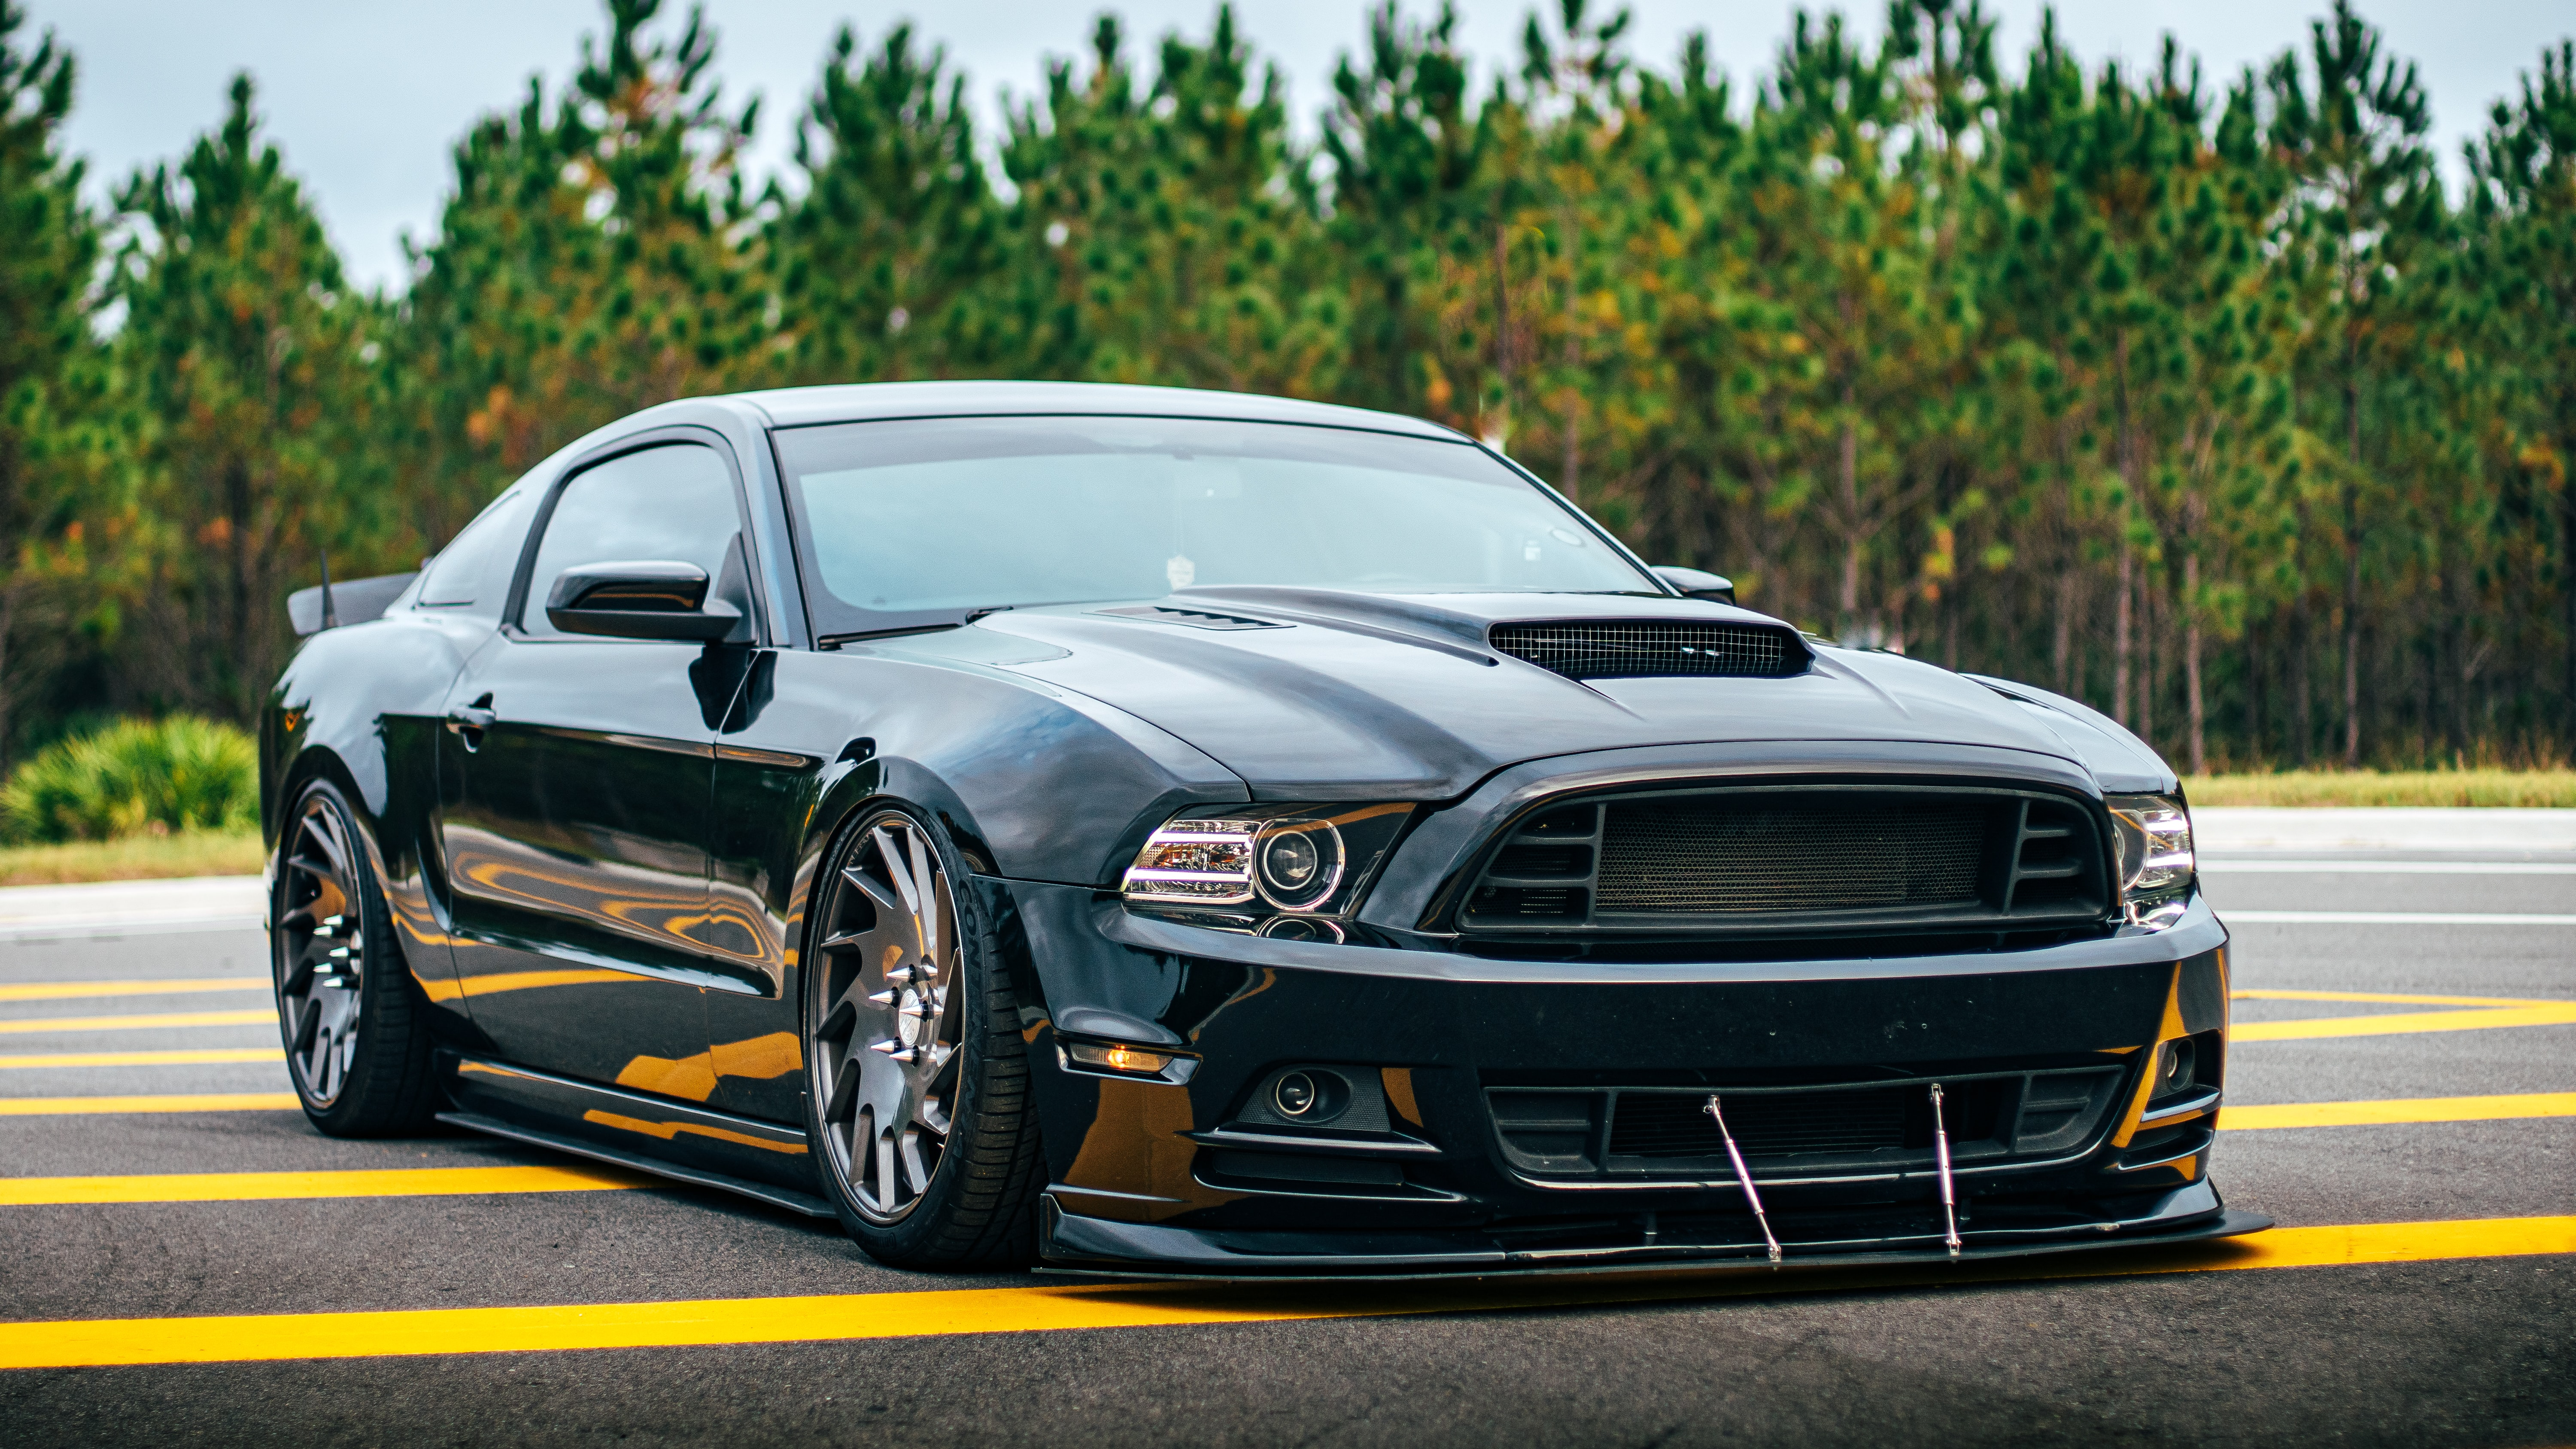
\includegraphics[keepaspectratio=true,scale=0.38]{2.png}} 
		\captionof{figure}{Description d'une offre}\label{f3}%
\end{page}
\end{page}
\subsection{Maquette 6}
\begin{page}{\textwidth}
	\begin{page}{\linewidth}
	\makebox[\linewidth]{
		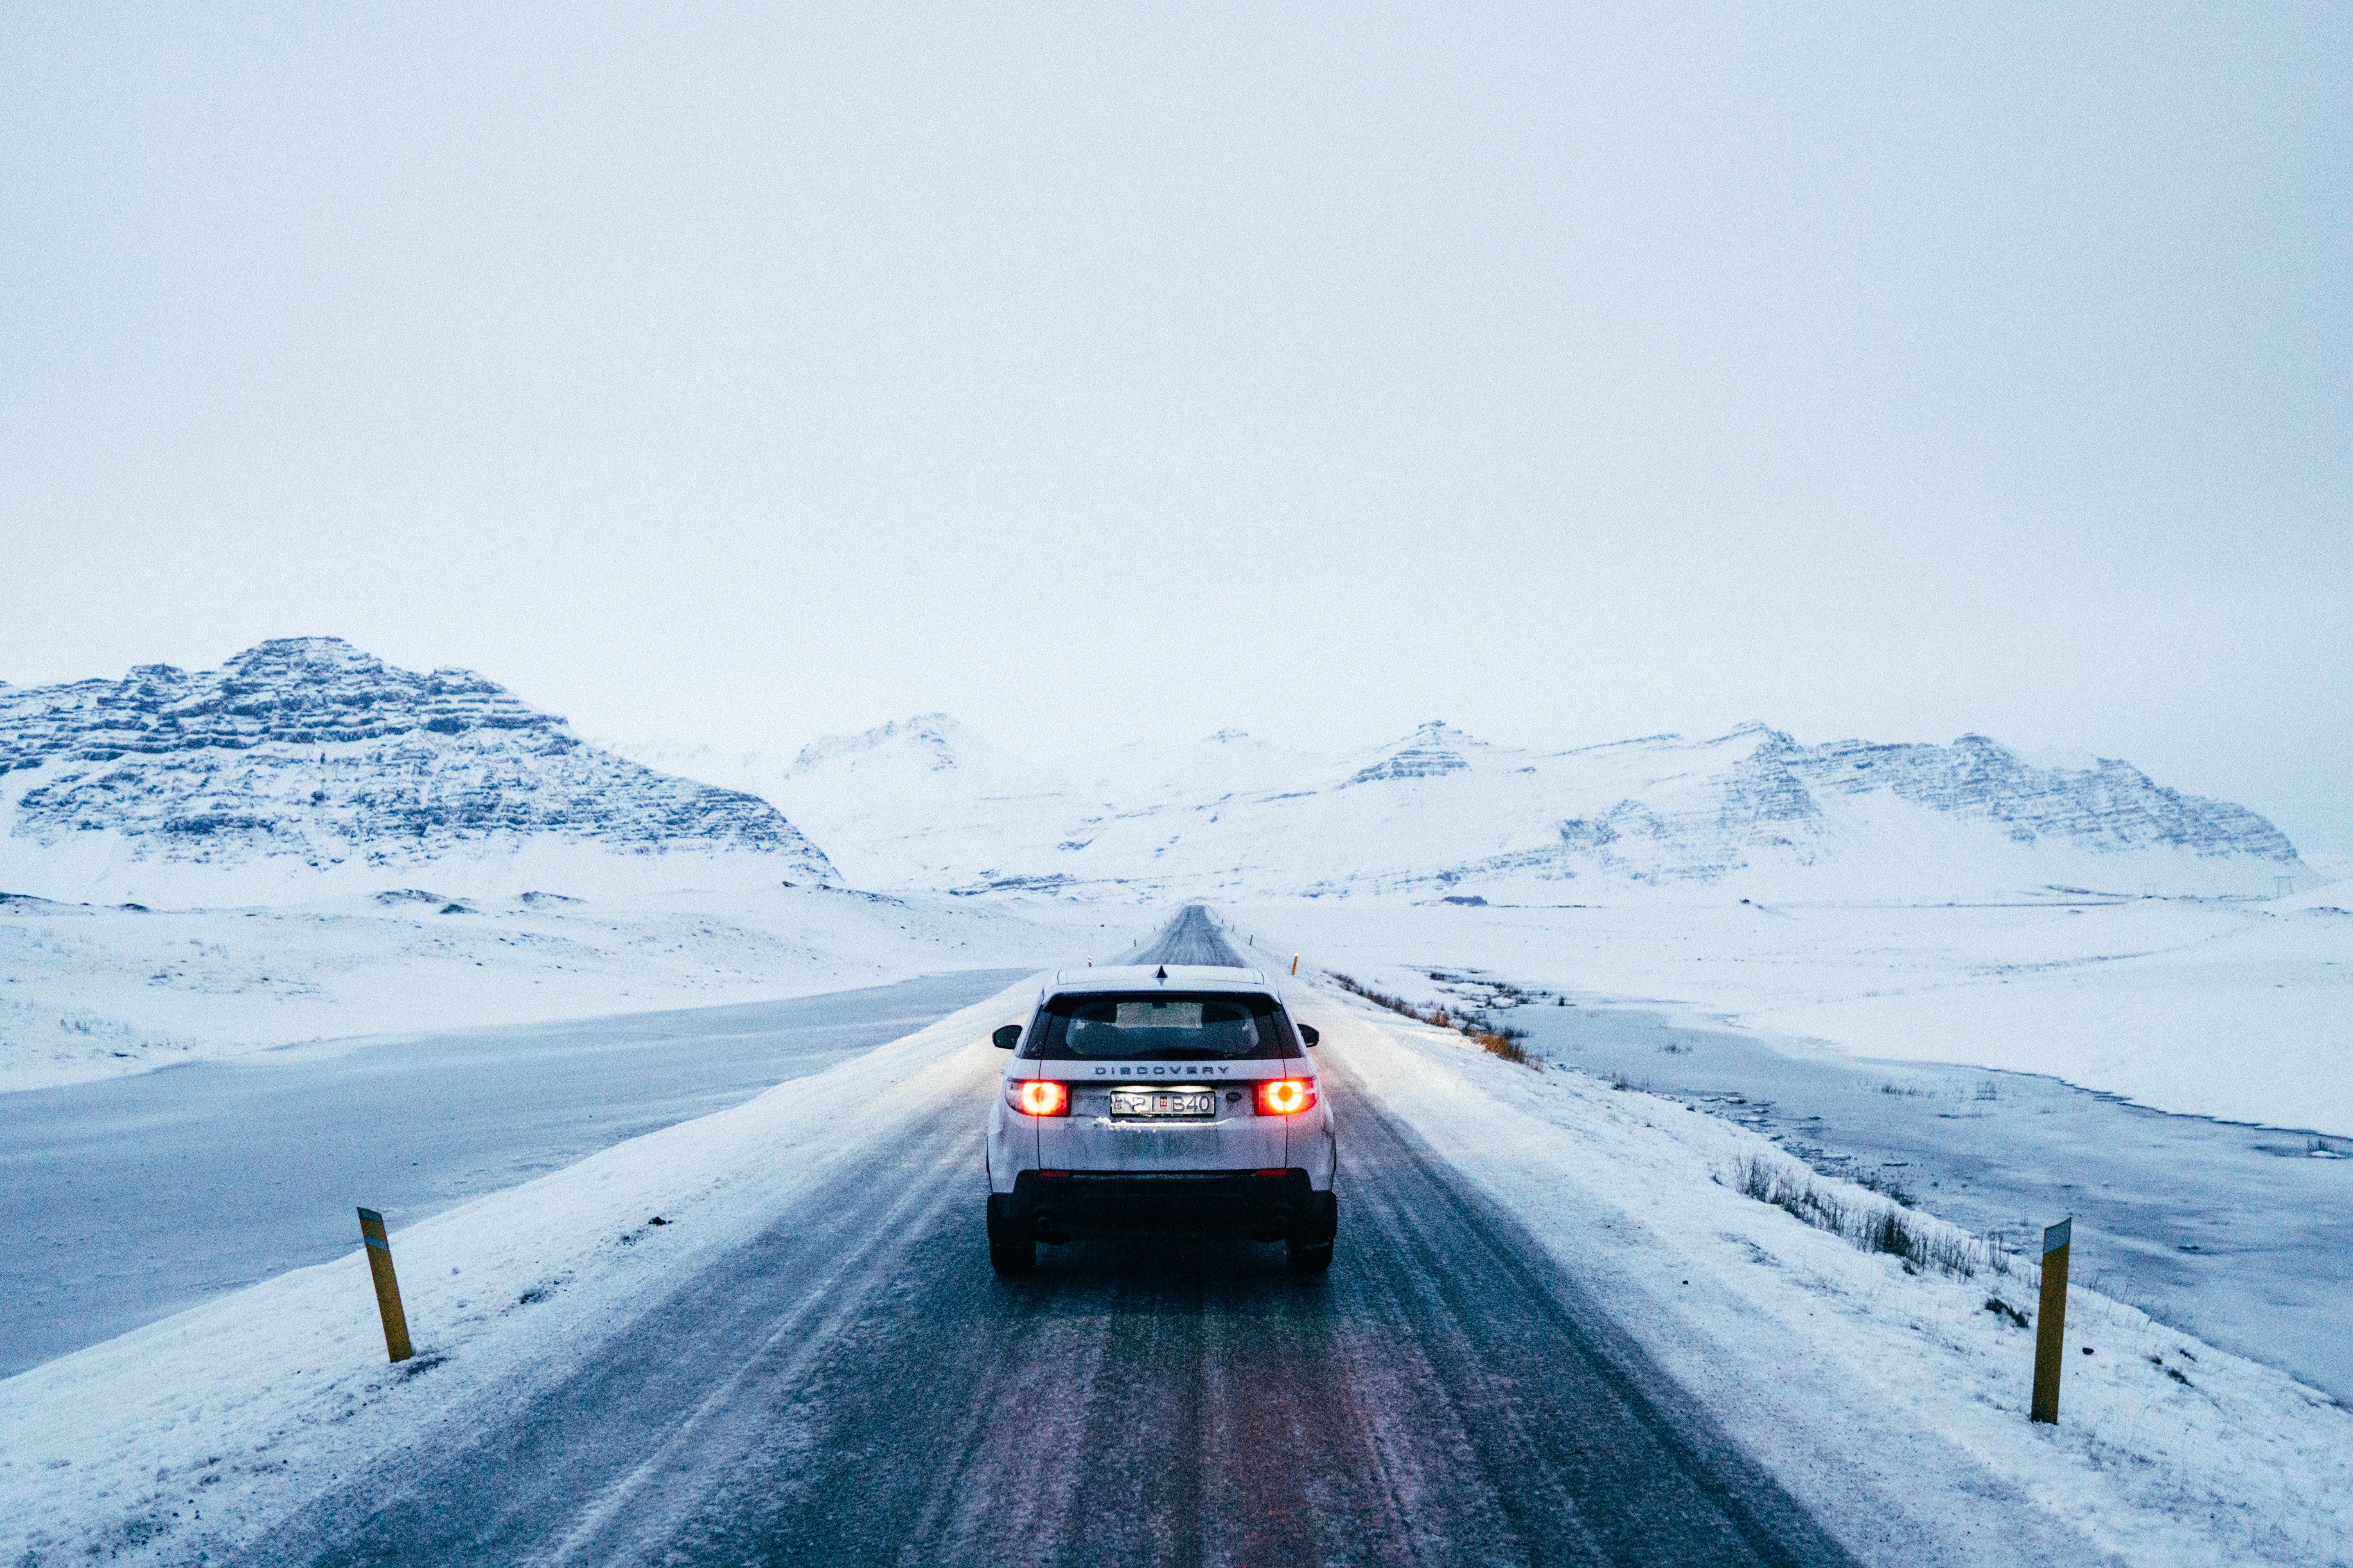
\includegraphics[keepaspectratio=true,scale=0.36]{3.png}} 
		\captionof{figure}{Créer une offre}\label{f3}%
\end{page}
\end{page}






\chapter{Réalisation}
\vspace{5cm}
\large{Ce dernier chapitre présente les spécifications des environnements matériels et logiciels utiliséesau cours du développement et aussi présente les différentes interfaces.\\}


\newpage

\section{les outils et les technologies}

\subsection{Pattern MVC}
Le pattern d'architecture logicielle MVC (\textbf{M}odèle-\textbf{V}ue-\textbf{C}ontrôleur) est un modèle destiné à répondre aux besoins des applications interactives en séparant les problématiques liées aux différents composants au sein de leur architecture respective..
Ce paradigme regroupe les fonctions nécessaires en trois catégories :\\
\begin{itemize}
\item[•] Un modèle : modèle de données.
\item[•] Une vue : interface utilisateur.
\item[•] Un contrôleur : logique de contrôle.\vspace{0.1cm}\\
\end{itemize}

\begin{minipage}{\linewidth}
	\makebox[\linewidth]{
		\includegraphics[keepaspectratio=true,scale=0.45]{mvc10}}
	\captionof{figure}{Pattern MVC.}\label{f3}%    
\end{minipage}\\



\subsection{Outils de développement }
\subsubsection{Langage de programmation}
\begin{minipage}{0.18\textwidth}
	\begin{minipage}{\linewidth}
	\makebox[\linewidth]{
		\includegraphics[keepaspectratio=true,scale=0.4]{jee}} 
		\captionof{figure}{Java EE}\label{f3}%
\end{minipage}
\end{minipage}
\hfill
\begin{minipage}{0.75\textwidth}
(Java Entreprise Edition) est la version entreprise de la plate-forme "Java" qui se compose de l'environnement "JSE" ainsi que de nombreuses API et composants destinés à une utilisation "côté serveur" au sein du système d'information de l'entreprise.\\

\textbf{\textit{Justification:}} JAVA est sécurisée, il a été conçu pour être exploité dans des environnements serveur et distribués. Dans ce cadre, la sécurité n’a pas été négligeable. C’est le langage le plus adopté par les développeurs grâce à sa fiabilité et sa performance élevé. \\
\end{minipage}\\

\subsubsection{Environnement de  développement}
\begin{minipage}{0.2\textwidth}
	\begin{minipage}{\linewidth}
		\makebox[\linewidth]{
			\includegraphics[keepaspectratio=true,scale=0.4]{eclipse.png}} 
			\captionof{figure}{eclipse}\label{f3}%
	\end{minipage}
\end{minipage}
\hfill
\begin{minipage}{0.75\textwidth}
	Eclipse est un environnement de développement intégré pour des applications open source et multi-plateformes. Cela fonctionne principalement comme plateforme de programmation, et il peut compiler et déboguer beaucoup de langues de programmation: bien qu'ils soit plus connu pour la programmation dans Java, sa modularité te permet de l'utiliser pour la programmation en C, Python...\\
	
	\textbf{\textit{Justification:}} Un démarrage rapide et une prise en main progressive,. Un scope fonctionnel complet et une productivité accrue.\\
\end{minipage}\\
\subsubsection{Gestion de version \& collaboration:}
\begin{minipage}{0.2\textwidth}
	\begin{minipage}{\linewidth}
		\makebox[\linewidth]{
			\includegraphics[keepaspectratio=true,scale=0.12]{git}}  
			\captionof{figure}{git}\label{f3}%
	\end{minipage}
\end{minipage}
\hfill
\begin{minipage}{0.75\textwidth}
	Git est un logiciel de gestion de versions décentralisé. C'est un logiciel libre créé par Linus Torvald, auteur du noyau Linux, et distribué selon les termes de la licence publique générale GNU version 2. En 2016, il s’agit du logiciel de gestion de versions le plus populaire qui est utilisé par plus de douze millions de personnes.\\
\end{minipage}\\

\begin{minipage}{0.2\textwidth}
	\begin{minipage}{\linewidth}
		\makebox[\linewidth]{
			\includegraphics[keepaspectratio=true,scale=0.04]{github}} 
			\captionof{figure}{github}\label{f3}%
	\end{minipage}
\end{minipage}
\hfill
\begin{minipage}{0.75\textwidth}
GitHub est un service web d'hébergement et de gestion de développement de logiciels, utilisant le logiciel de gestion de versions Git. Ce site est développé en Ruby on Rails et Erlang par Chris Wanstrath, PJ Hyett et Tom Preston-Werner. GitHub propose des comptes professionnels payants, ainsi que des comptes gratuits pour les projets de logiciels libres. Le site assure également un contrôle d'accès et des fonctionnalités destinées à la collaboration comme le suivi des bugs, les demandes de fonctionnalités, la gestion de tâches et un wiki pour chaque projet.\\
\end{minipage}\\

\subsubsection{Design \& Multimédia:}
\begin{minipage}{0.2\textwidth}
	\begin{minipage}{\linewidth}
		\makebox[\linewidth]{
			\includegraphics[keepaspectratio=true,scale=0.3]{html}}  
			\captionof{figure}{html}\label{f3}%
	\end{minipage}
\end{minipage}
\hfill
\begin{minipage}{0.75\textwidth}
	L'HyperText Markup Language, généralement abrégé HTML, est le langage de balisage conçu pour représenter les pages web. C'est un langage permettant d'écrire de l'hypertexte, d'où son nom.\\
\end{minipage}\\

\begin{minipage}{0.2\textwidth}
	\begin{minipage}{\linewidth}
		\makebox[\linewidth]{
			\includegraphics[keepaspectratio=true,scale=0.04]{css}}
			\captionof{figure}{css}\label{f3}%
	\end{minipage}
\end{minipage}
\hfill
\begin{minipage}{0.75\textwidth}
	Les feuilles de style en cascade, généralement appelées CSS de l'anglais Cascading Style Sheets, forment un langage informatique qui décrit la présentation des documents HTML et XML. Les standards définissant CSS sont publiés par le World Wide Web Consortium.\\
\end{minipage}\\
\begin{minipage}{0.28\textwidth}
	\begin{minipage}{\linewidth}
		\makebox[\linewidth]{
			\includegraphics[keepaspectratio=true,scale=0.31]{js}}   
			\captionof{figure}{JavaScript}\label{f3}%
	\end{minipage}
\end{minipage}
\hfill
\begin{minipage}{0.75\textwidth}
	JavaScript (qui est souvent abrégé en « JS ») est un langage de script léger, orienté objet, principalement connu comme le langage de script des pages web.\\
\end{minipage}\vspace{0.5cm}\\
\begin{minipage}{0.2\textwidth}
	\begin{minipage}{\linewidth}
		\makebox[\linewidth]{
			\includegraphics[keepaspectratio=true,scale=0.18]{eee}}  
			\captionof{figure}{jstl}\label{f3}%
	\end{minipage}
\end{minipage}
\hfill
\begin{minipage}{0.75\textwidth}
	La JavaServer Pages Standard Tag Library est un composant de la plate-forme JEE de développement. Elle étend la spécification JSP en ajoutant une bibliothéque de balises pour les taches courantes, comme le travail sur des fichiers XML, l'exécution conditionnelle, les boucles et l'internationalisation.
\end{minipage}\vspace{0.5cm}\\
\subsubsection{Serveur d’application:}
\begin{minipage}{0.2\textwidth}
	\begin{minipage}{\linewidth}
		\makebox[\linewidth]{
			\includegraphics[keepaspectratio=true,scale=0.31]{tomcat}}   
			\captionof{figure}{Tomcat}\label{f3}%
	\end{minipage}
\end{minipage}
\hfill
\begin{minipage}{0.75\textwidth}
	Tomcat est un conteneur web libre de servlets et JSP. Issu du projet Jakarta, c'est un des nombreux projets de l’Apache Software Foundation.\\
\end{minipage}\\


\section{ Présentation de Louezz}

Cette partie dénombre la présentation des Scénarios applicatifs de l'application. Nous allons présenter dans ce qui suit, les imprimes-écran des principales interfaces réalisées dans notre site web.
\subsection{Page d'accueil}

C'est la page d'accueil qui s'affiche dès l'accès à notre site web, elle est constituée de trois parties principales :\\

• Un champ de recherche donnant aux visiteurs de notre plateforme le choix de sélection des offres selon la ville et la date de disponibilité.\\

• Un slider animé donnant un flash sur les dernieres offres\\



\begin{minipage}{\linewidth}
	\makebox[\linewidth]{
		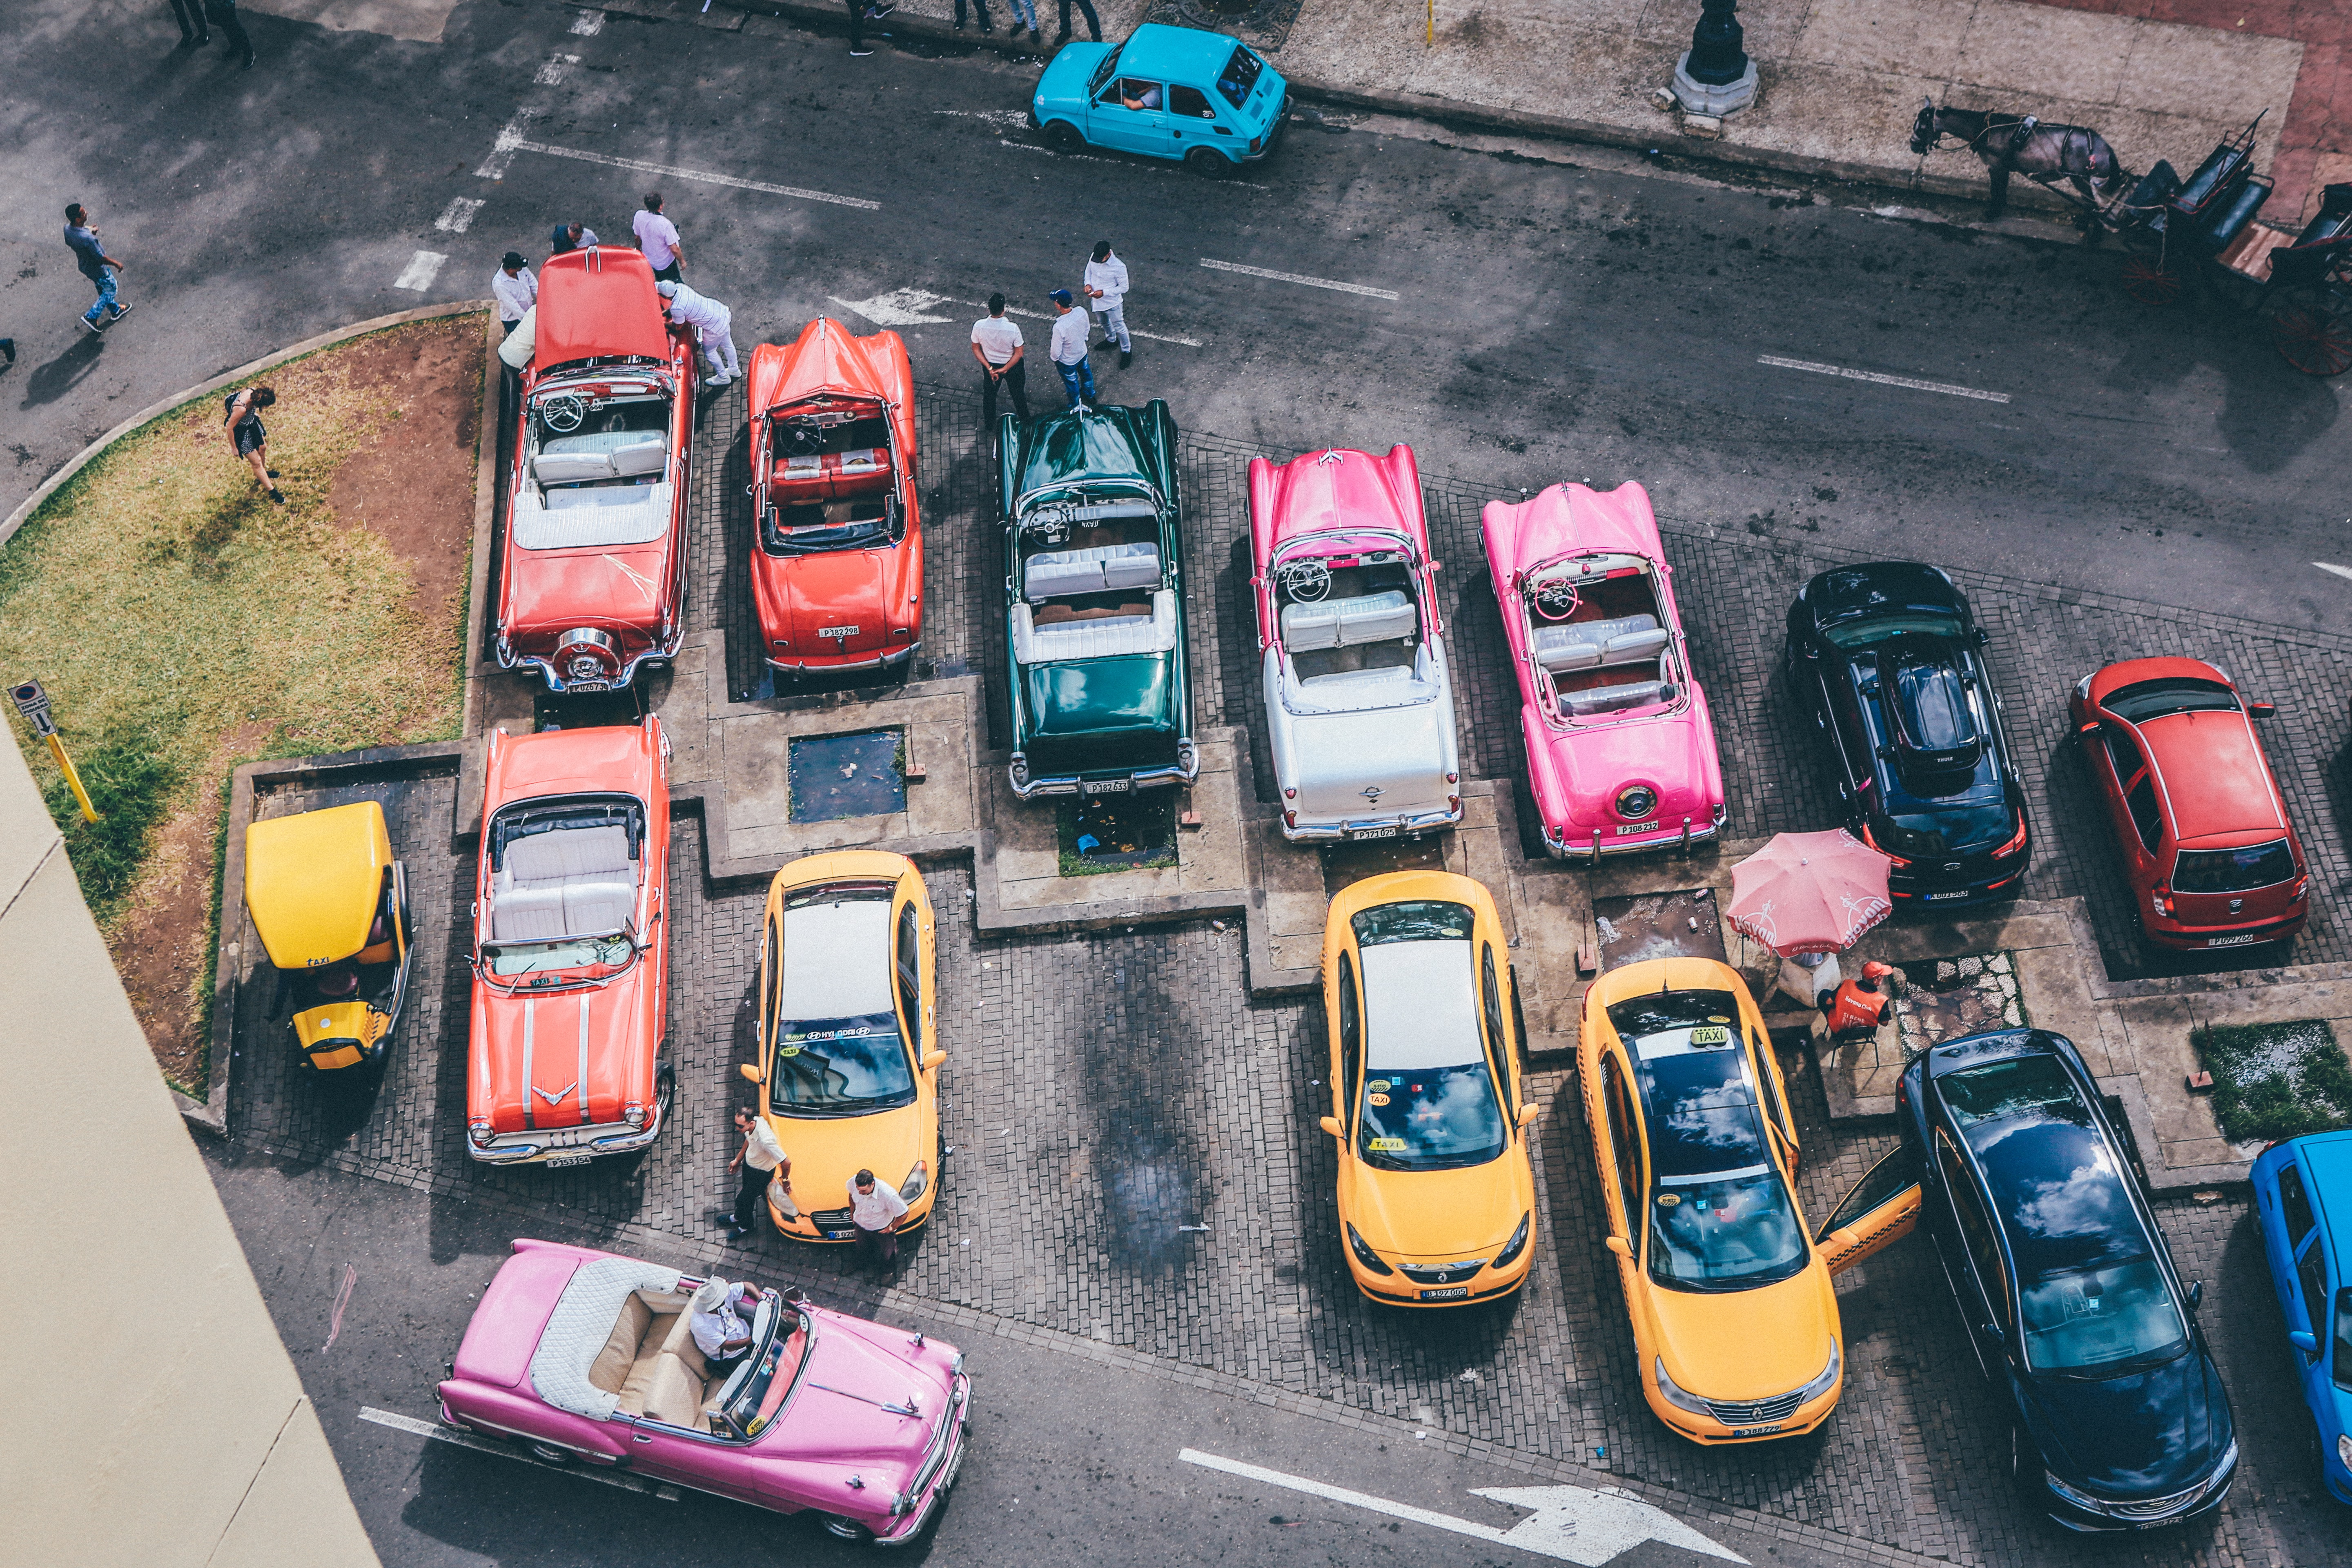
\includegraphics[keepaspectratio=true,scale=0.25]{1.jpeg}}
	\captionof{figure}{Page d'aceuil}\label{f3}%    
\end{minipage}\\


\begin{minipage}{\linewidth}
	\makebox[\linewidth]{
		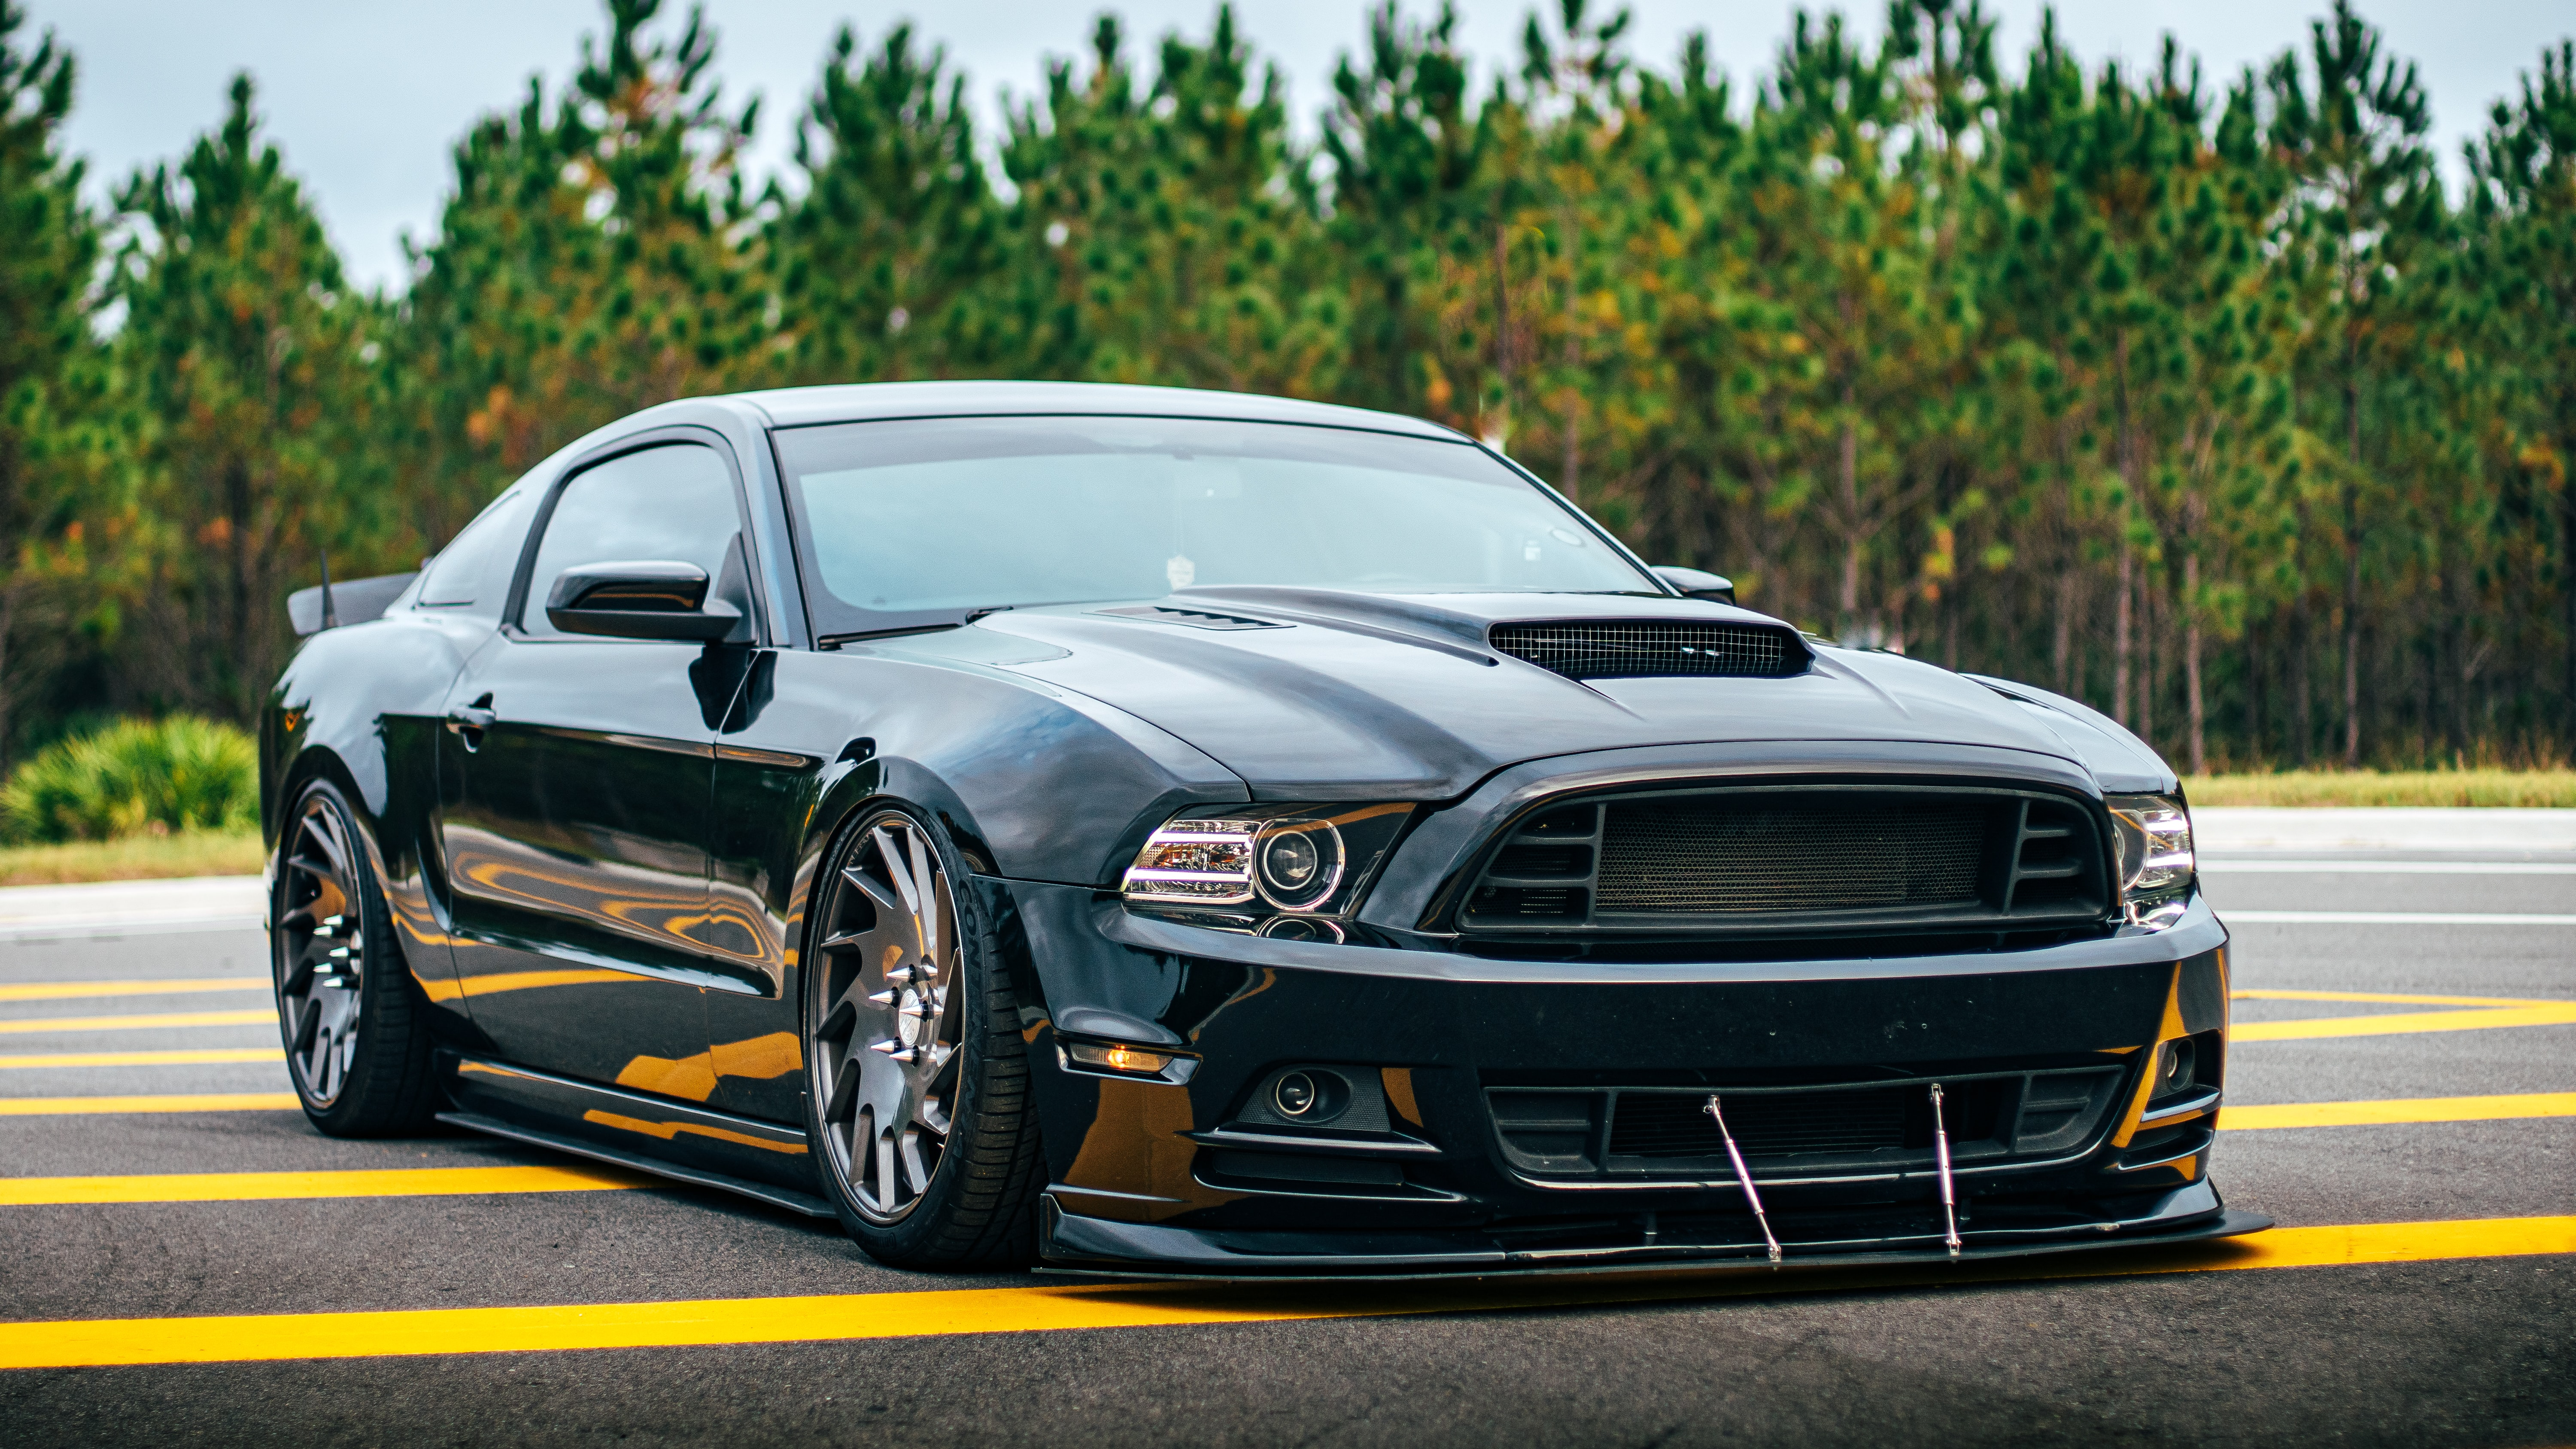
\includegraphics[keepaspectratio=true,scale=0.25]{2.jpeg}}
	\captionof{figure}{Page d'ajout de voiture}\label{f3}%    
\end{minipage}\\


\begin{minipage}{\linewidth}
	\makebox[\linewidth]{
		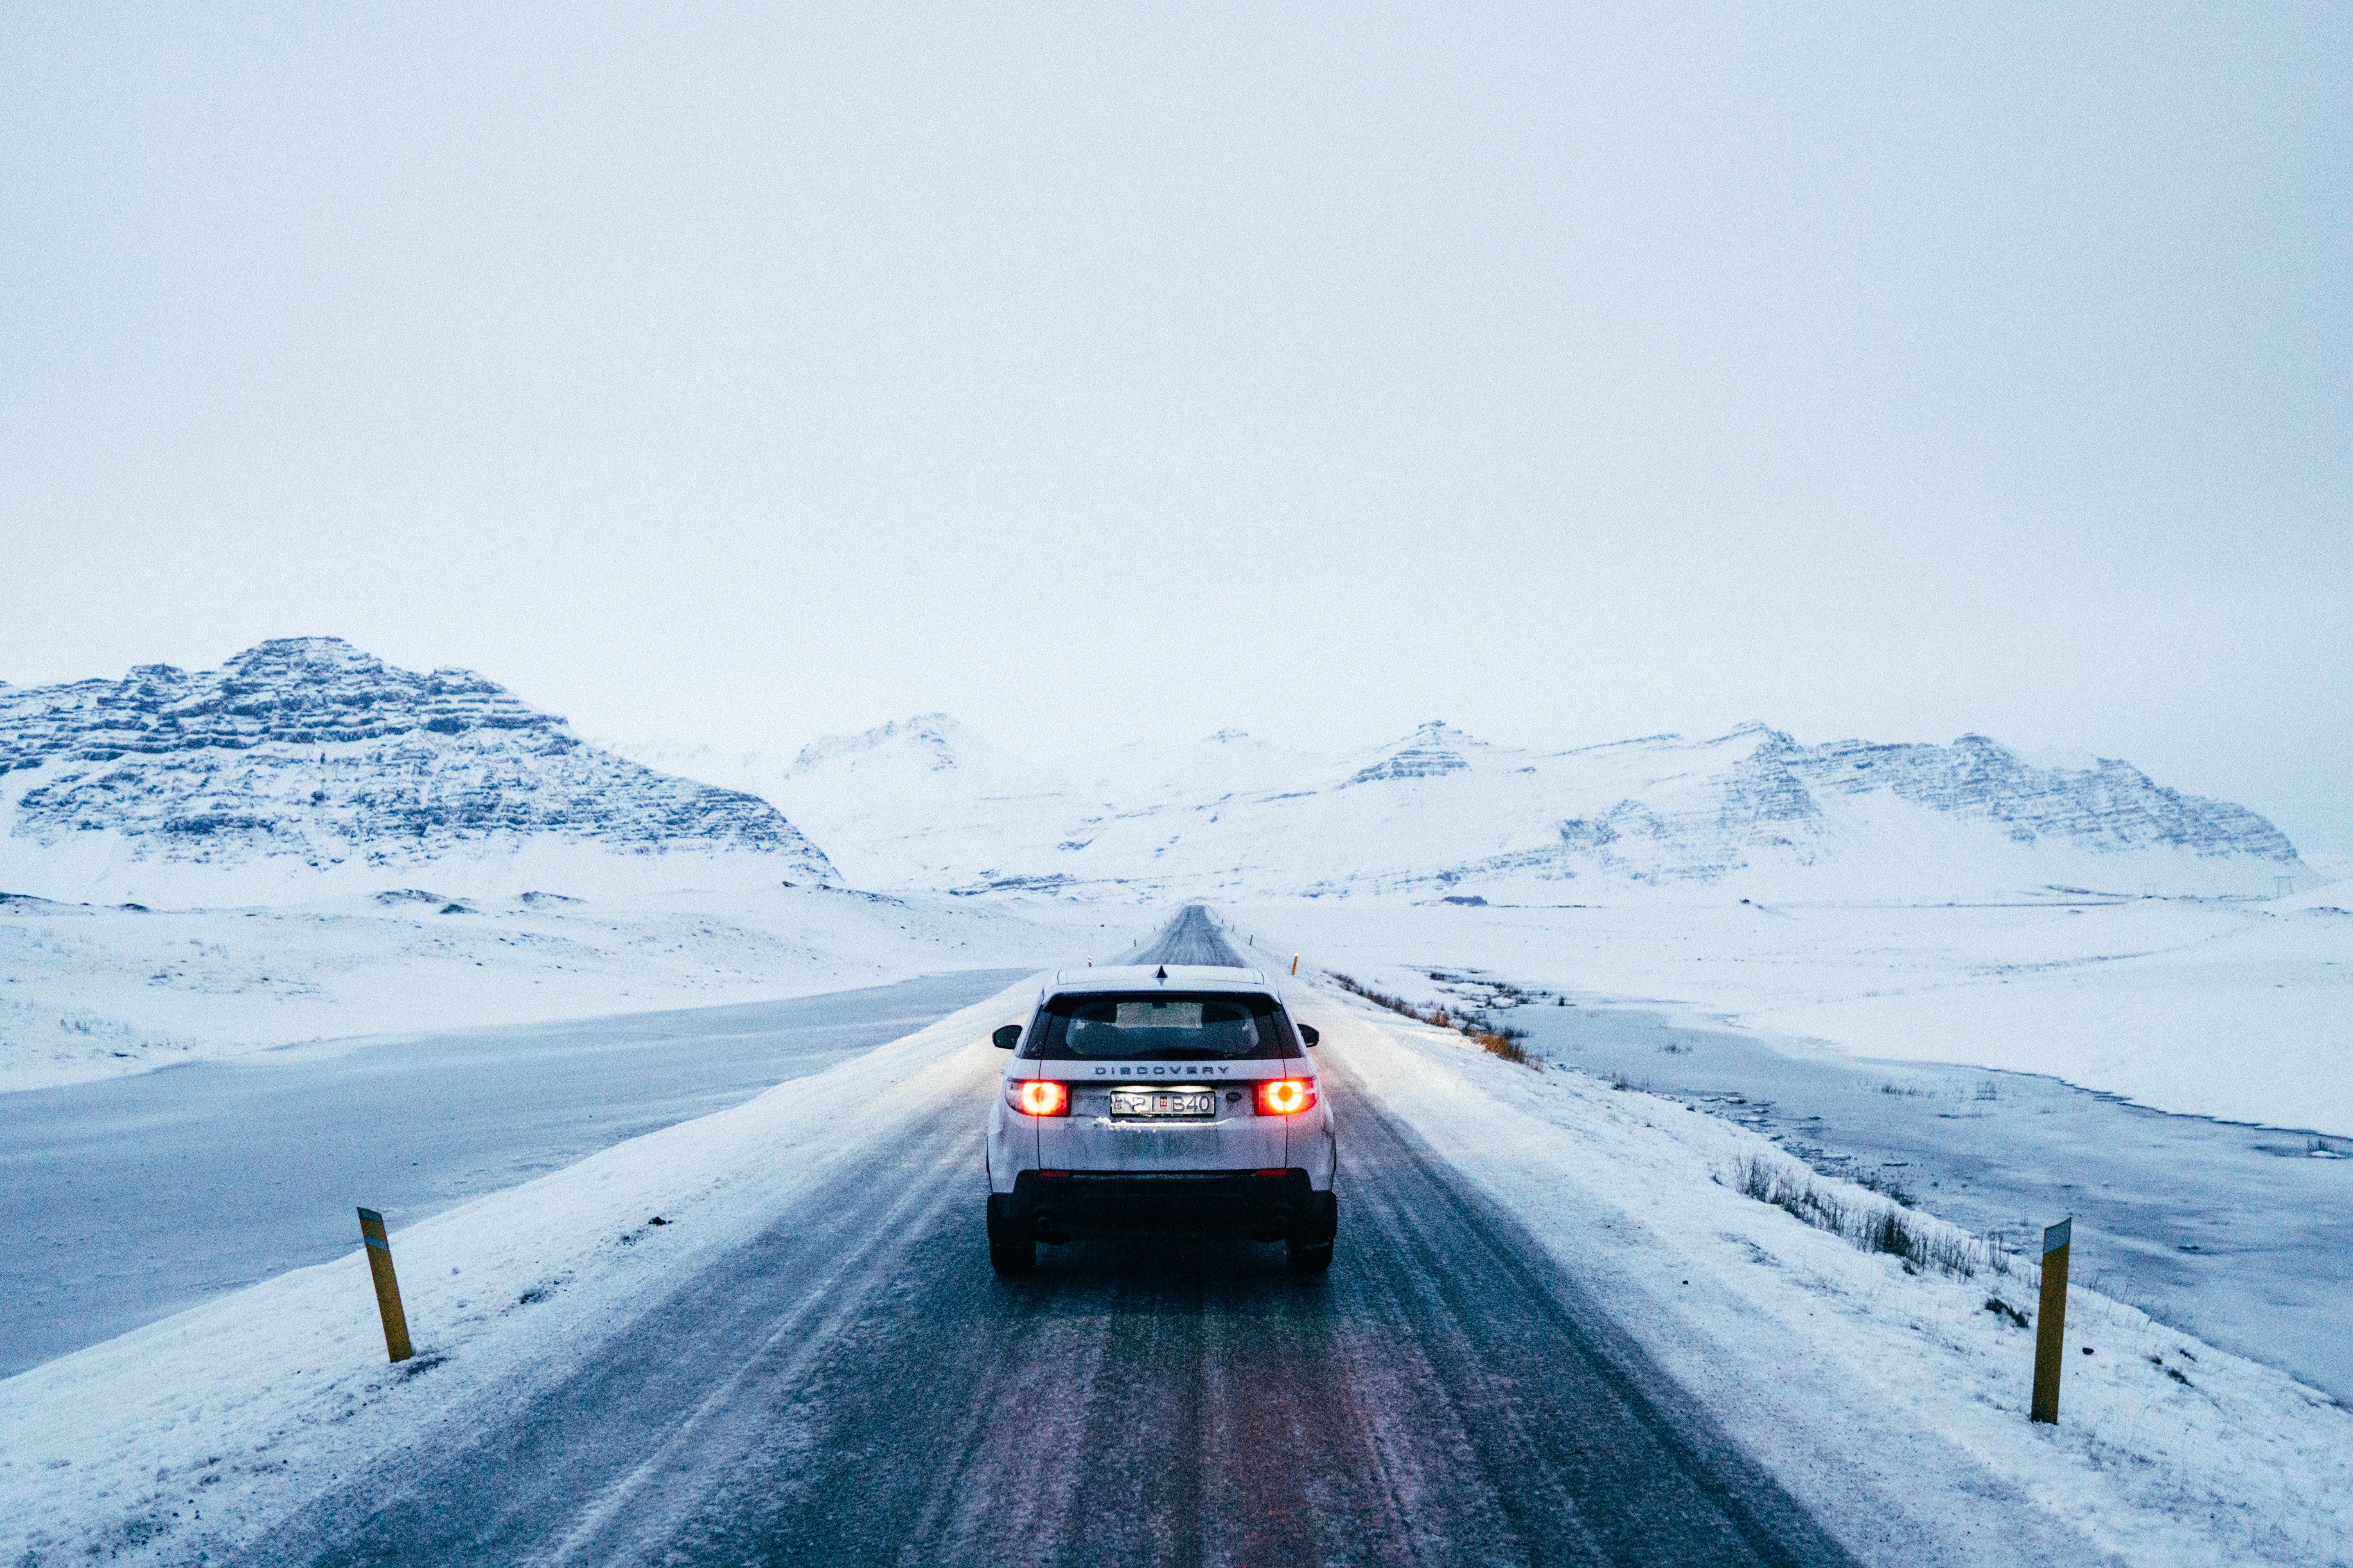
\includegraphics[keepaspectratio=true,scale=0.25]{3.jpeg}}
	\captionof{figure}{Page d'affichage d'offre}\label{f3}%    
\end{minipage}\\


\begin{minipage}{\linewidth}
	\makebox[\linewidth]{
		\includegraphics[keepaspectratio=true,scale=0.25]{4.jpeg}}
	\captionof{figure}{Page de detail d'offfre}\label{f3}%    
\end{minipage}\\

\begin{minipage}{\linewidth}
	\makebox[\linewidth]{
		\includegraphics[keepaspectratio=true,scale=0.25]{5.jpeg}}
	\captionof{figure}{Page de d'affichage de mes voitures}\label{f3}%    
\end{minipage}\\

\begin{minipage}{\linewidth}
	\makebox[\linewidth]{
		\includegraphics[keepaspectratio=true,scale=0.25]{6.jpeg}}
	\captionof{figure}{Page de modification des donnees de ma voiture}\label{f3}%    
\end{minipage}\\

\begin{minipage}{\linewidth}
	\makebox[\linewidth]{
		\includegraphics[keepaspectratio=true,scale=0.25]{7.jpeg}}
	\captionof{figure}{Page de profile}\label{f3}%    
\end{minipage}\\

\begin{minipage}{\linewidth}
	\makebox[\linewidth]{
		\includegraphics[keepaspectratio=true,scale=0.25]{8.jpeg}}
	\captionof{figure}{Page de changement de mot de passe}\label{f3}%    
\end{minipage}\\

\begin{minipage}{\linewidth}
	\makebox[\linewidth]{
		\includegraphics[keepaspectratio=true,scale=0.25]{9.jpeg}}
	\captionof{figure}{  Page de modification des données de mon profile}\label{f3}%    
\end{minipage}\\
\begin{minipage}{\linewidth}
	\makebox[\linewidth]{
		\includegraphics[keepaspectratio=true,scale=0.25]{11.jpeg}}
	\captionof{figure}{  Page de connexion}\label{f3}%    
\end{minipage}\\


\begin{minipage}{\linewidth}
	\makebox[\linewidth]{
		\includegraphics[keepaspectratio=true,scale=0.25]{12.jpeg}}
	\captionof{figure}{  Page d'inscription}\label{f3}%    
\end{minipage}\\

\begin{minipage}{\linewidth}
	\makebox[\linewidth]{
		\includegraphics[keepaspectratio=true,scale=0.25]{13.jpeg}}
	\captionof{figure}{
	Page de demandes ou cas d'inexistance des demandes
	}\label{f3}%    
\end{minipage}\\

\begin{minipage}{\linewidth}
	\makebox[\linewidth]{
		\includegraphics[keepaspectratio=true,scale=0.25]{14.jpeg}}
	\captionof{figure}{Page de mes voitures
	
	}\label{f3}%    
\end{minipage}\\

\begin{minipage}{\linewidth}
	\makebox[\linewidth]{
		\includegraphics[keepaspectratio=true,scale=0.25]{15.jpeg}}
	\captionof{figure}{Page de done}\label{f3}%    
\end{minipage}\\

\begin{minipage}{\linewidth}
	\makebox[\linewidth]{
		\includegraphics[keepaspectratio=true,scale=0.25]{10.jpeg}}
	\captionof{figure}{Page des erreurs}\label{f3}%    
\end{minipage}\\
\chapter*{Conclusion générale}
\addcontentsline{toc}{chapter}{Conclusion générale}
Tout au long de ce rapport, nous avons présenté les différentes étapes de la réalisation de l’application du projet. Pour le développement de ce projet nous avons utilisé le langage UML, ce qui a permis de mener correctement la tâche d’analyse des besoins à l’aide du diagramme de cas d’utilisation et la tâche de conception, ainsi les scénarios sont aussi détaillés afin d’expliquer toutes les tâches faites puisque nous travaillons avec la technologie JEE.\\

Ce projet nous a permis de développer nos compétences techniques, d’approfondir
nos connaissances théoriques et pratiques, de stimuler un esprit d’initiative et de
créativité, et notamment dans le domaine de développement des applications web.
Il nous a donné la méthode pour assurer un travail de groupe, comment compter sur
soi pour résoudre les problèmes au cas où ils se présentent, comment être professionnels dans notre travail, comment être attentifs aux indications de notre encadrant, comment être bien organisés pour accomplir dans les meilleurs délais, et meilleures conditions les tâches qui nous sont confiées. Ce projet nous a donné l’occasion de faire le lien entre les connaissances académiques, notamment en JAVA, Base de Données et le monde professionnel.\\

Notre application peut être aisément améliorée grâce à son aspect ouvert. Dans notre application, nous avons travaillé dans un réseau local. Pour la mettre en ligne nous avons seulement besoin de l’héberger sur un serveur.\\
\chapter*{Webographie}
\addcontentsline{toc}{chapter}{Webographie}
[1] \href{https://openclassrooms.com/fr/courses/626954-creez-votre-application-web-avec-java-ee}{https://openclassrooms.com/fr/courses/626954-creez-votre-application-web-avec-java-ee}\\

[2] \href{https://docs.oracle.com/javaee/7/index.html}{https://docs.oracle.com/javaee/7/index.html}\\

[3] \href{https://www.supinfo.com/articles/single/3099-waterfall-model-modele-cascade}{https://www.supinfo.com/articles/single/3099-waterfall-model-modele-cascade}\\

[4] \href{http://www.uml-sysml.org/documentation}{ttp://www.uml-sysml.org/documentation} \\

[5] \href{https://www.supinfo.com/articles/single/2519-architecture-client-serveur}{https://www.supinfo.com/articles/single/2519-architecture-client-serveur}    
 \\  





%espacement entre les lignes d'un tableau
\renewcommand{\arraystretch}{1.5}

%====================== INCLUSION DES PARTIES ======================

~
\thispagestyle{empty}
\newpage


\end{document}